\chapter{Particioniranje prostora}
Kako smo to spomenuli u uvodu, postoje razni algoritmi za detekciju sudara. Najvažniji od njih su oni kojima dijelimo objekte (BVH), i one kojima dijelimo prostor. Algoritam s kojim dijelimo objekt smo već prošlu u poglavlju \ref{cha:BVH}. Kako smo u nekom trenutku odustali od BVH-a bilo je potrebno pronaći dobar i brz način za detektiranje sudara na cijeloj sceni. Detekcija sudara sama po sebi, komplicirana je operacija i potrebno je da bude manje složena od O(n\texttt{$^2$}) operacija. Kako smo to opisali u poglavlju \ref{cha:BVH}, BVH-u je ptorebno O{logN} operacija sa detekciju sudara na sceni, iako je nekada prije potrebno napraviti dodatne kalkulacije i ažuriranja strukture da bi ona bila funkcionalna. To dodatno komplicira stvari, ali je vrlo efikasno. U ovom poglavlju, pokazati ćemo da je particioniranje prostora također jedna efikasna i lako razumljiva strategija za detekciju sudara.

\section{Primitivna detekcija sudara}
U prošlom poglavlju objasnili smo kako sudare, nakon što ih detektiramo, kalkulirati. Nigdje nismo spomenuli kako smo i te sudare detektirali. Koristili smo za to vrlo primitivan i jednostavan algoritam. Za svaki objekt na sceni, iterativno bi tražili s kojim se objektom sudara. Ovo u principu nije problem kada je situacija sa zidovima jer u konačnici imamo 4 zida pa je sama složenost te operacije O(4 * N). Problem se javlja kada imamo kuglica. Do 50 kuglica ovaj algoritam će raditi, no nakon prelaska na veći broj kuglica javlja se problem. Za 500 kuglica potrebno je napraviti isto toliko provjera. To nas dovodi do brojke od 250 000 tisuća provjera i složenosti O(n\texttt{$^2$}). Kako smo ranije opisali ovo smo željeli izbjeći. Takav algoritam bi glasio ovako:
\begin{algorithm}
	\caption{Algoritam za primitivnu detekciju sudara između kuglica}
	\label{alg:primitive_collision}
	\begin{algorithmic}
		\Function {searchCollisions}{$Ball$ $list[N]$}
		\State $i = 1$
		\For {$ball$ in $list$}
		\While{$i < N$}
		\If {$ifCollision(ball, list[i])$}
		\State $resolveCollision(ball,list[i])$
		\EndIf
		\State $i++$
		\EndWhile
		\EndFor
		\EndFunction
	\end{algorithmic}
\end{algorithm}
gdje je:
\begin{itemize}
	\item list - lista kuglica
	\item N - broj kuglica
\end{itemize}
Kako smo ranije već spomenuli, za listu smo koristili \emph{std::vector} u C++. Ovakav pristup smo koristili samo pri početku projekta. Za mali broj kuglica i za provjeru ispravnosti proračuna, ovakav pristup je bio dovoljan. \newpage
\section{k-d stablo (K-dimensional tree)}
Spomenuli smo da je složenost koju želimo postići pri detektiranju sudara najmanje O(NlogN) (za N objekata na sceni). Da bi to postigli moramo naš prostor podijeliti u smislene regije u kojima ćemo provjeravati sudar. Promotrimo to na jednom primjeru:
\begin{figure}[!http]	
	\begin{center}
		\begin{tikzpicture}
		\draw (0,-2) rectangle (10,10);
		\draw (5,4) circle(0.7) node {1};
		\draw (9,6) circle(0.7) node {3};
		\draw (4,7) circle(0.7) node{2};
		\draw (8,1) circle(0.7) node {5};
		\draw (7,2) circle(0.7) node {4};
		\draw (2,3) circle(0.7) node {6};
		\end{tikzpicture}
	\end{center}
	\caption{Primjer kuglica na sceni}
	\label{fig:26}
\end{figure}\newline
gdje su koordinate centara:\newpage
\begin{itemize}
	\item 1 - (5,4)
	\item 2 - (4,7)
	\item 3 - (9,6)
	\item 4 - (7,2)
	\item 5 - (8,1)
	\item 6 - (2,3)
\end{itemize}
Na slici \ref{fig:25} vidimo da ne treba u svim situacijama provjeravati sudar. Na primjer za kuglicu 2 i 6 znamo da se sudar neće dogoditi te tu provjeri ne moramo uzimati u obzir dok između kuglica 5 i 4 te 1 i 2 znamo da bi se mogao dogoditi sudar u skorom vremenu, te, te sudare moramo provjeriti.

Postoje mnoge tehnike za podijeliti prostor, no ona koju smo mi koristili je k-d stablo. k-d stablo je binarno stablo gdje je svaki čvor k-dimenzionalna točka\cite{14}. Svaki čvor koji nije list, može se shvatit kao ravnina koja dijeli prostor. Točke koje se nalaze lijevo od ravnine predstavlja lijeva strana stabla, dok desne točke predstavlja desna strana stabla\cite{14}. Konkretno, ukoliko odaberemo X os za os podijele, točke manje od vrijednosti X bit će nam u lijevoj grani stabla, dok točke veće od X vrijednosti će biti na desnoj strani stabla\cite{14}. U 3D prostoru intuitivno je da ćemo imat 3 dimenzije. Dakle, root čvor stabla će podijeliti prostor prema X koordinati, zatim njegova djeca prema Y koordinati, djeca djece po Z koordinati itd. .
\begin{figure}[!http]
	\begin{center}
		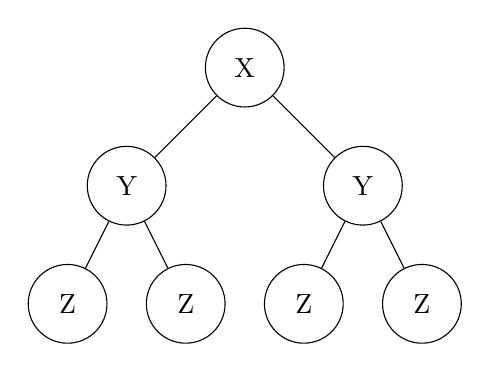
\begin{tikzpicture}[level distance=1.5cm,
		level 1/.style={sibling distance=3cm},
		level 2/.style={sibling distance=1.5cm}]
		\node[draw, circle,inner sep=1pt, minimum size = 1cm] {X}
		child {node[draw, circle,inner sep=1pt, minimum size = 1cm] {Y}
			child {node[draw, circle,inner sep=1pt, minimum size = 1cm] {Z}}
			child {node[draw, circle,inner sep=1pt, minimum size = 1cm] {Z}}
		}
		child {node[draw, circle,inner sep=1pt, minimum size = 1cm] {Y}
			child {node[draw, circle,inner sep=1pt, minimum size = 1cm] {Z}}
			child {node[draw, circle,inner sep=1pt, minimum size = 1cm] {Z}}
		};
		
		\end{tikzpicture}
	\end{center}
	\caption {Prikaz k-d stabla za 3 dimenzije}
	\label{fig:25}
\end{figure} \newline
Nakon što smo došli do Z dimenzije, ponovno dijelimo prostor po "x" koordinati, i tako se vrtimo dok ne podijelimo cijeli prostor. 
Sada se možemo vratiti na situaciju iz slike \ref{fig:26}. k-d stablo će nam onakav prostor podijeliti na sljedeći način\cite{14}:
\begin{figure}[!http]
	\begin{center}
		\begin{tikzpicture}
		\draw (0,0) rectangle (10,10);
		\draw (5,4) circle(0.7) node {1};
		\draw[blue] (0,4) -- (7,4);
		\draw (9,6) circle(0.7) node {3};
		\draw[blue] (7,6) -- (10,6);
		\draw (4,7) circle(0.7) node{2};
		\draw[red] (4,4) -- (4,10);
		\draw (8,1) circle(0.7) node {5};
		\draw[red] (8,0) -- (8,6);
		\draw (7,2) circle(0.7) node {4};
		\draw[red] (7,0) -- (7,10);
		\draw (2,3) circle(0.7) node {6};
		\draw[red] (2,0) -- (2,4);
		\tkzInit[xmax=10,ymax=10,xmin=-2,ymin=-2]
		\tkzAxeXY

		\end{tikzpicture}
	\end{center}
	\caption {Podjela prostora k-d stablom}
	\label{fig:27}
\end{figure}\newline
Primjetimo da smo prostor podijelili po koordinatama centra svake kuglice.Crvene linije prikazuju podjelu prostora po X koordinati, dok plave ukazuju na podjelu prostora po Y koordinati. Da smo imali još Z koordinatu, analogija je ista, imali bi dodatnu dimenziju, no zbog jednostavnosti dovoljno je ovo prikazati u 2D prostoru.\newpage

\subsection{Izgradnja k-d stabla}
U prijašnjem poglavlju podijelili smo prostor bez da znamo zapravo kako je to napravljeno niti da znamo kako će struktura stabla izgledati za takvu situaciju. Općenito, znamo kako struktura stabla izgleda. Svaka razina stabla particionirala je prostor po nekoj koordinati. Jedino pitanje koje se postavlja je, kako izabrati točke na način da dobijemo kvalitetno podijeljen prostor i balansirano stablo. S obzirom da postoji puno načina na koji možemo odabrati osi presijecenja koje su poravnate s koordinatnim osima, postoji i puno načina da izgradimo k-d stablo. Kanonski način izgradnje je onaj koji smo već opisali\cite{14}:
\begin{itemize}
	\item Kako se krećemo po stablu, kružno biramo osi presijecanja
	\item Točke odabiremo tako da odaberemo median element s obzirom na os presijecanja
\end{itemize}
Ovakva metoda će nas dovesti do balansiranog stabla, iako za sve aplikacije to nije nužan uvjet \cite{14}.

S obzirom na sve ovo možemo napisati jednostavan algoritam za izgradnju samog k-d stabla.

\begin{algorithm}
	\caption{Algoritam za izgradnju k-d stabla\cite{14}}
	\label{alg:k-d_tree_build}
	\begin{algorithmic}
		\Function {K-d tree}{$Point$ $pointList[N]$, $depth$}
		\State $axis = depth\mod{k}$ 
		\State $Sort(list)$
		\State Select $median$ by $axis$ from $pointList$
		\State $Node.point = median$
		\State $Node.left(pointList[0...Median-1], depth+1)$
		\State $Node.right(pointList[Median+1...pointList.size], depth+1)$
		\EndFunction
	\end{algorithmic}
\end{algorithm}
\newpage
Sada kada znamo izgraditi stablo možemo prikazati kako bi stablo konkretno izgledalo za situaciju na slici \ref{fig:27} it prošlog poglavlja:
\begin{figure}[!http]
	\begin{center}
		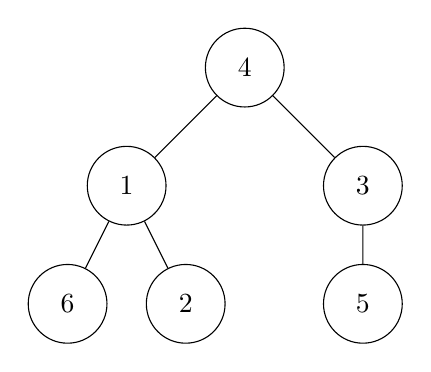
\begin{tikzpicture}[level distance=1.5cm,
		level 1/.style={sibling distance=3cm},
		level 2/.style={sibling distance=1.5cm}]
		\node[draw, circle,inner sep=1pt, minimum size = 1cm] {4}
		child {node[draw, circle,inner sep=1pt, minimum size = 1cm] {1}
			child {node[draw, circle,inner sep=1pt, minimum size = 1cm] {6}}
			child {node[draw, circle,inner sep=1pt, minimum size = 1cm] {2}}
		}
		child {node[draw, circle,inner sep=1pt, minimum size = 1cm] {3}
			child {node[draw, circle,inner sep=1pt, minimum size = 1cm] {5}}
		};
		
		\end{tikzpicture}
	\end{center}
	\caption {Prikaz strukture k-d stabla za sliku \ref{fig:27}}
	\label{fig:28}
\end{figure}
Prikažimo ovo isto stablo sa koordinatama centara\cite{14}:
\begin{figure}[!http]
	\begin{center}
		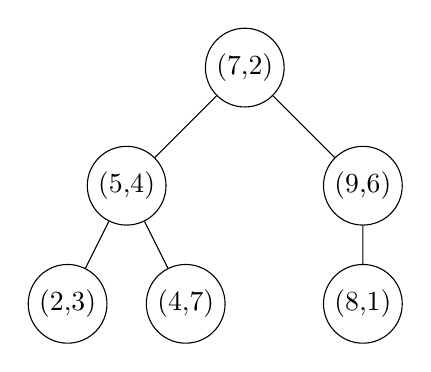
\begin{tikzpicture}[level distance=1.5cm,
		level 1/.style={sibling distance=3cm},
		level 2/.style={sibling distance=1.5cm}]
		\node[draw, circle,inner sep=1pt, minimum size = 1cm] {(7,2)}
		child {node[draw, circle,inner sep=1pt, minimum size = 1cm] {(5,4)}
			child {node[draw, circle,inner sep=1pt, minimum size = 1cm] {(2,3)}}
			child {node[draw, circle,inner sep=1pt, minimum size = 1cm] {(4,7)}}
		}
		child {node[draw, circle,inner sep=1pt, minimum size = 1cm] {(9,6)}
			child {node[draw, circle,inner sep=1pt, minimum size = 1cm] {(8,1)}}
		};
		
		\end{tikzpicture}
	\end{center}
	\caption {Prikaz strukture k-d stabla za sliku \ref{fig:27}}
	\label{fig:28-1}
\end{figure}

Složenost ovog algoritma ovisi o složenosti operacije sortiranja i pretrage za median elementom. Pozicija median elementa se pronalazi kao:
\begin{equation}
	Median =\frac{N}{2}
\end{equation}
gdje je:
\begin{itemize}
	\item N - broj elemenata
\end{itemize}
Algoritmi koji se uglavnom koriste za sortiranje su \emph{Mergesort} (implementiran u C++ STL-u) i \emph{Heapsort}. Složenost ovih algoritama u općem slučaju je O(NlogN). Sukladno tome to je i najbolja složenost koja se može postići s ovim algoritmima sortiranja. Složenost izgradnje stabla u najgorem slučaju može biti O(kNlogN) operacija što ćemo mi i imati s obzirom da u svakoj od k dimenzija moramo sortirati točke i odabrati median element. S obzirom da se kuglice na sceni kreću, stablo moramo graditi u svakom frameu pa je i ovakav način detekcije sudara sam po sebi dosta složen, no još uvijek je brži od onog opisanog u algoritmu \ref{alg:primitive_collision}. 

Sada kada smo naš prostor podijelili prema točkama kuglica, potrebno je samo pretražiti sve potencijalne sudare na sceni. Dobra osobina k-d stabla je ta što će nam podijeliti prostor po gustoći točaka. Tako možemo vrlo jednostavno detektirati sudare na sceni i izračunati ih ukoliko se sudar dogodio.

\subsection{Pretraga sudara u k-d stablu}
Pretraga sudara u k-d stablu nakon izgradnje je trivijalna stvar. Sve se svodi na jednostavno šetanje po stablu. Da dodatno ne povećavamo složenost, šetanje će uključiti samo onu granu stabla koja je bliže u prostoru i/ili onu s kojom se kuglica sudara. Da se izbjegne korištenje funkcije korijena (\emph{sqrt}) koristiti će se kvadrirana udaljenost (eng. \emph{squared distance}). Ukoliko detektiramo sudar, u istom trenutku ga i računamo. Algoritam je rekurzivan i glasi:\newpage
\begin{algorithm}
	\caption{Algoritam za pretragu sudara u k-d stablu}
	\label{alg:serch_collisions_kd}
	\begin{algorithmic}	
		\Function {searchCollisions}{$Ball ball$, $K-dTreeNode Node$}
		\If {$Node$ is leaf}
		\If {$isCollision(ball, node)$}
		\State $resolveCollision(ball,node)$
		\EndIf
		\Return
		\EndIf
		\If {$isCollision(ball, node)$}
			$resolveCollision(ball,node)$
		\EndIf
		\If{$distance(Node.left,ball) > distance(Node.right,ball)$ or
		\State $isCollision(ball, node.right)$}
		\State $searchCollisions(ball, node.right)$
		\ElsIf{$distance(Node.right,ball) > distance(Node.left,ball)$ or \State $isCollision(ball, node.left)$}
		\State $searchCollisions(ball, node.left)$
		\EndIf
		\EndFunction
		
		\Function {checkAllBalls}{$Ball listBall[N]$, $K-dTreeNode Node$}
		\For {$ball$ in $listBall$}
		\State $searchCollisions(ball,Node)$
		\EndFor
		\EndFunction

	\end{algorithmic}
\end{algorithm}
Na ovakav ćemo način vrlo jednostavno na cijeloj sceni detektirati sudare i izračunati. S obzirom da je kuglica uvijek u sudaru sama sa sobom, potrebno je izbjeći računanje takvog sudara. Prilikom implementacije klase za kuglice, u kodu \ref{code:7}, spomenuli smo atribut \emph{i} tipa integer. Ovaj atribut označava poziciju kuglice u listi i na taj način ćemo vrlo jednostavno izbjeći računanje sudara kuglice same sa sobom. Testiranjem je utvrđeno da se prilikom takvog računanja mogu pojaviti anomalije i ponašanje kuglica koje ne želimo.\newpage
\subsection{Implementacija klase za k-d stablo}
U ovome poglavlju nećemo prikazivati implementaciju svih funkcija. Opisati ćemo samo odluke i strukturu same klase.
\begin{lstlisting}[style = myC++, label = {code:13}, caption={Implementacija klase za k-d stablo}]

template <class T> class KDtreeNode {
static bool sortbyX(T lhs, T rhs) 
static bool sortbyY(T lhs, T rhs) 
static bool sortbyZ(T lhs, T rhs) 

public:
	KDtreeNode *left()
	KDtreeNode *right() 
	unsigned long childSize() 
	unsigned int getPlane()
	void build_tree(std::vector<T> &v, int depth) 
	void treeTraverse() 
	template <class T1> void searchCollisions(T1 &ball)
private:
	std::vector<KDtreeNode> child;
	T object;
	unsigned int plane;
};

\end{lstlisting}

U početku bila je dilema koristiti li normalnu klasu koja bi radila samo an temelju kuglica, ili \emph{template} klasu koja bi onda radila za sve tipove objekata koje bi stavili scenu. Odabrana je \emph{template} klasa upravo iz tog razloga, da prilikom dodavanja nekih drugih objekata koji nisu kuglice, ne moramo raditi novu strukturu za samo taj specifični objekt. Točnost ove tvrdnje pokazana je kada se ista klasa za k-d stablo koristila i za particioniranje zidova. Jednom strukturom smo odradili posao za sve moguće objekte na sceni. Postoji i bolji pristup da se koriste samo točke objekata, ali za nas je ovakav bio dovoljan. Klase \emph{sortby(x,y,z)} poslužile su za sortiranje cijele liste prema određenoj osi. Ostale funkcije koje smo koristili su ili već opisane (\emph{build\texttt{\_}tree}, \emph{searchCollisions}) ili su samo \emph{Get} funkcije za dohvat privatnih varijabli. \newpage
\section{Prednosti i mane korištenja algoritama za particioniranje prostora (k-d stabla)}

K-d stablo svakako pronalazi svoju uporabu u stvarnome svijetu. Vrlo jednostavna implementacija i razumijevanje same strukture omogućuje široku primjenu u svijetu igara. Skladno tome, jasno je da je k-d stablo dobar način kojim ćemo pretraživati sudare na sceni. Vrlo je efikasno iako ima svoje mane. 

Prva od njih je ta da u svakom koraku izgradnje stabla moramo sortirati cijelu listu točaka i to nam uvijek zahtjeva najmanje O(NlogN) operacija. Na taj način smo ograničeni i tu ne možemo napraviti dodatne optimizacije iako one postoje. Postoji bolji način odabira ravnine presjecanja i točke koja će biti čvor (npr. metoda fiksne točke ili odabir slučajne točke)\cite{14}. Ove metode nam ipak neće dati balansirano stablo, ali to s druge strane ovisi o našim potrebama. Balansirano stablo u praksi nije uvijek prijeko potrebno pa se možemo spasiti od silnog sortiranja u svakom koraku izgradnje stabla. 

S druge strane, ukoliko nam treba balansirano stablo, sortiranje ne možemo izbjeći. Zato se k-d stablo u praksi često koristi za statične objekte koji se ne gibaju\cite{14}. Tako možemo izvršiti izgradnju stabla prije pokretanja animacije. Dobar primjer iskorišten je i kod nas gdje smo izgradili stablo od zidova. Iako zida postoje samo 4 na sceni, zgodno je bilo pokazati da je k-d stablo zapravo puno efikasnije kod statičnih objekata.

Kod kuglica se događao problem s velikim brojem kuglica (500+), jer unutar 30-60 FPS-a nismo uspjeli izvršiti sve provjere sudara i izračunati iste. Ovdje se može uvesti jedna optimizacija da se u svakoj pretragi sudara računa i vrijeme do idućeg sudara, no mi je nismo koristili.


